\chapter{Implementáció}
\label{cha:implementation}

A komponensek fejlesztésekor Eclipse fejlesztő környezetet használtam, verziókezeléshez pedig a Git szoftvert. Az alapértelmezett Eclipse IDE azonban nem tökéletes eszköz az OSGi alapú fejlesztéshez, ezért a Bndtools \cite{bndtools} OSGi fejlesztő keretrendszert Eclipse kiegészítő modulként feltelepítve kezdtem neki a komponensek fejlesztésének.

\section{WikiBot bundle}
\label{sec:wikibotbundle}

A WikiBot komponens architektúráját teljes mértékben a fejlesztéskor használt IRC Bot készítő keretrendszerek határozták meg. A kezdeti változatban a PircBot \cite{pircbot} keretrendszert használtam, azonban hosszan tartó használata alatt kiderült, hogy a rendszernek több hibája is van. Hosszabb ideig tartó futáskor ismeretlen eredetű hibák kerültek elő a PircBot könyvtárban, melyek okait a rossz tervezés miatt felderíteni sem volt lehetséges. A keretrendszert Java 1.1 verzióra tervezték, nem használja ki az azóta a nyelvben megjelent újdonságokat, így teljesen elavultnak számít technológiailag, hiába fejlesztik azóta folyamatosan. A hibák nagyon sok esetben teljesen elnyelődnek a rendszerben, így sok esetben lehetetlen az alkalmazás hibáinak megfejtése. Egyes metódusok, melyek örökléskor felüldefiniálva jól használhatóak lennének, private vagy final hozzáférés-vezérlési kulcsszavakkal vannak ellátva. További rossz tervezési döntés a God Object antipatternnel való visszaélés.

Ezen hátrányok miatt egy idő után az újabb, kevésbé elterjedt, de jobban karbantartott verziójára tértem át a PircBot-nak, mely a PircBotX \cite{pircbotx} nevet viseli. Ez a váltás azonban csak kis mértékben befolyásolta a fejlesztés menetét, hiszen mindkét keretrendszernél egy esemény alapú architektúra kialakítása szükséges, melyben különféle események esetén implementálni kell a rendszer viselkedését.

A bundle-ök implementációja során a komponensek függőségeinek, melyek külső könyvtárakban voltak, szintén el kellett készíteni a bundle változatait, hogy azok hiánya ne jelentkezzen hibaként az OSGi függőségkezelőjében. Ez a lépés mind a PircBot, mind a PircBotX esetén a külső könyvtárak OSGi komponens formára való alakítását jelentette, melyet a Bndtools nevű eszközzel hajtottam végre. Ebben a lépésben gyakorlatilag a kész JAR kiterjesztésű library-t kellett egy OSGi specifikáció szerint meghatározott manifest állománnyal újracsomagolni.

\begin{figure}[htp]
\centering
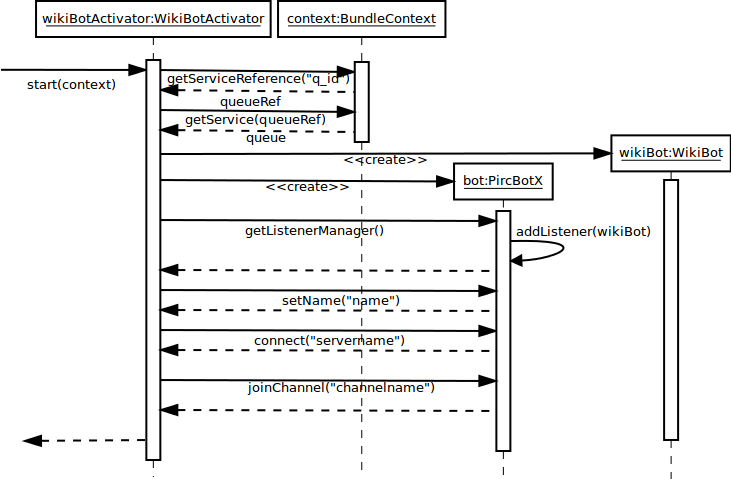
\includegraphics[scale=0.5]{img/sequence_wikiBot}
\caption{WikiBot komponens indulása}
\label{fig:sequence_wikiBot}
\end{figure}

A komponens működése látható a \ref{fig:sequence_wikiBot}.~ábrán: először el kell kérni a QueueManager referenciáját, majd egy PircBotX példányhoz hozzá kell adni egy Listener-t, amely implementálja az eseménykezelőt függvényeket. Ezután meg kell adni az IRCBot nevét, csatlakozni kell egy szerverhez, végül be kell lépni egy IRC csatornába. Ettől a ponttól kezdve, ha egy üzenet érkezik a csatornába (\ref{fig:sequence_wikiBot2}.~ábra), a WikiBot kiszedi a szükséges információkat reguláris kifejezésekkel és elhelyezi a QueueManager-ben.

\begin{figure}[htp]
\centering
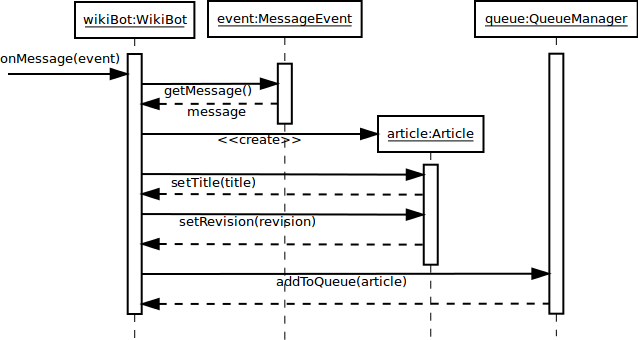
\includegraphics[scale=0.5]{img/sequence_wikiBot2}
\caption{Eseménykezelés a WikiBot-ban}
\label{fig:sequence_wikiBot2}
\end{figure}

% section wikibotbundle (end)

\section{Parser bundle}
\label{sec:parserbundle}

Az összes komponens közül a Parser felépítése a legösszetettebb, többszálú működése miatt egyszerre történik sok minden, ezért a működésen keresztül fogom bemutatni, hogy teljesíti a Parser a tervezésben meghatározottakat.

A komponens indulásakor először megszerzi a kiajánlott adatbázis szolgáltatás referenciáját, a feldolgozás után itt fogja eltárolni a feldolgozott cikkeket azok adataival. Létrehoz ezenkívül egy QueueManager-t, beállít (.addObserver() metódus) számára egy újonnan létrehozott megfigyelőt (WikiObserver osztály), és beregisztrálja a queue-t, mint OSGi szolgáltatást. Végül ha elérhető Wikipedia adatbázis mentés (dump), akkor megkezdi annak feldolgozását is. Az indulás folyamata figyelhető meg a \ref{fig:sequence_parser}.~ábrán.

\begin{figure}[htp]
\centering
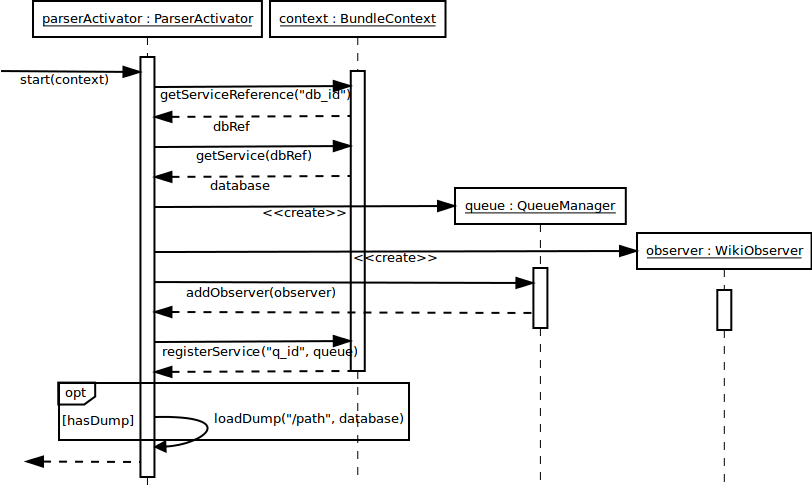
\includegraphics[scale=0.5]{img/sequence_parser}
\caption{A Parser komponens indulása}
\label{fig:sequence_parser}
\end{figure}

A cikkek feldolgozása külön szálakon történik meg, a minél gyorsabb működés érdekében. Minden cikkhez külön Thread objektum példányosítása rendkívül nagy overhead-del járna, ezért a \ref{cha:design} fejezetben már említett ThreadPool mintát használtam. Ez a minta a Thread objektumok újrahasznosításával működik, így nem szükséges mindig új szálat példányosítani. Használata a következő \ref{lst:threadpool}.~kódrészletben figyelhető meg, futtatáskor a szálak nevéből látszik, hogy mindig újrahasználjuk a kezdeti 10 darab szálat:

\begin{lstlisting}[label={lst:threadpool}, caption=ThreadPool használata,breaklines=true]
public class ThreadPoolExample {
    public static void main(String args[]){
       ExecutorService service = Executors.newFixedThreadPool(10);
       for (int i = 0; i < 100; i++){
           service.execute(new Runnable() {
        	   public void run() {
        		    System.out.println(Thread.currentThread().getName());
        			try {
						Thread.sleep(1000);
					} catch (InterruptedException e) {
						e.printStackTrace();
					}
        	   }   
           });
       }
    }
}
\end{lstlisting}

A Parser működése az eddigieket felhasználva a következő:

\begin{figure}[htp]
\centering
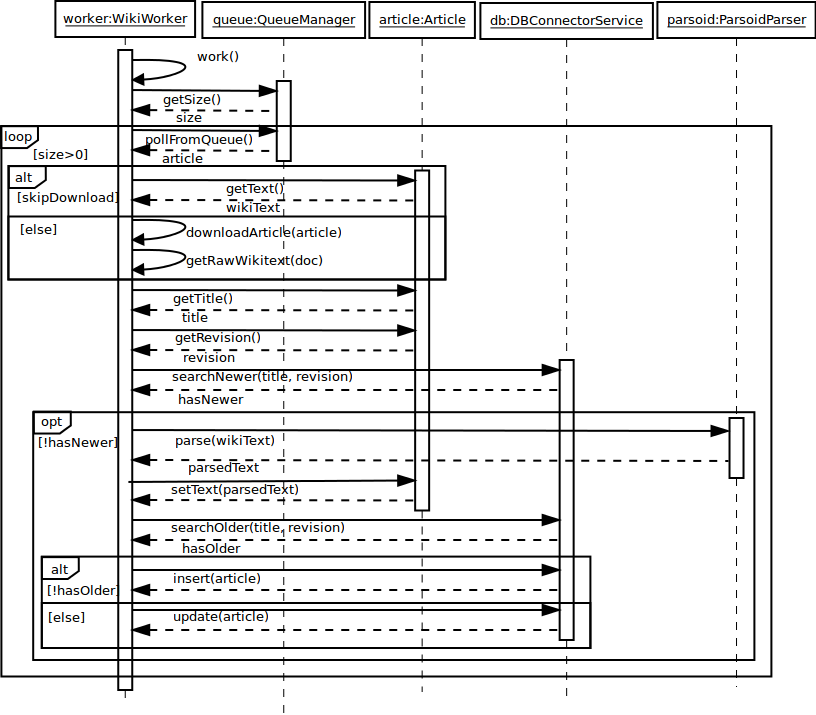
\includegraphics[scale=0.5]{img/sequence_parser2}
\caption{A WikiWorker szál működése}
\label{fig:sequence_parser2}
\end{figure}

\begin{enumerate}
	\item Ha egy új cikk kerül a QueueManager-be, akkor az Observer mintán keresztül a WikiObserver arról értesül.
	\item A WikiObserver egy új WikiWorker szálat rendel a ThreadPool-ból a feladathoz, mely megkezdi a cikk előfeldolgozását (\ref{fig:sequence_parser2}.~ábrán .work() metódus).
	\item A szál addig fut, amíg van feldolgozatlan cikk a queue-ban. A dump feldolgozásban fut a szál, akkor nem kell letölteni a cikkek szövegét, mert azokat ilyenkor a dump-ból már megszereztük. Ellenkező esetben le kell tölteni a hivatalos Wikipedia API-n keresztül a cikket XML formátumban, és ki kell szedni a Wikitext formátumban lévő szövegét.
	\item Ha van az adatbázisban már (.searchNewer() metódus) újabb verziójú cikk az adott cikkből, akkor nem kell tenni semmit, hiszen valószínűleg egy dump feldolgozásban vagyunk és korábban már on-the-fly megszereztük a cikk egy újabb verzióját.
	\item Ha nincs újabb verziójú cikk, akkor a Wikitext formátumról HTML (RDFa) formátumra kell alakítani a szöveget (.parse() metódus).
	\item Ha az adatbázisban van már régebbi verziójú cikk az adott cikkből, akkor valószínűleg on-the-fly feldolgozásban vagyunk és korábban már megszereztük a cikk egy korábbi verzióját. Ekkor az adatbázisban csak frissíteni kell a cikk adatait, máskülönben újonnan kell beilleszteni a cikket.
\end{enumerate}

Az előfeldolgozáskor kapott eredmények meghatározzák a feldolgozólánc használhatóságát, így fontos, hogy a megszerzett cikkek Wikitext formátumú szövegét milyen formában tároljuk. A \ref{cha:design}.~fejezetben láttuk, hogy a feldolgozáskor három cserélhető parser használható a rendszerben, melyek különböző képességekkel bírnak. Ezen parserek a Sztakipedia parser, DumbRegexWikipediaParser és a Parsoid parser. A Sztakipedia parser-nél szükség volt az MTA SZTAKI által készített Java nyelvű könyvtár OSGi komponenssé alakítására.

További felhasználás szempontjából a Parsoid készíti a legjobb kimenetet, azonban egyben a leglassabb is. Ezen lassúság kiküszöbölése miatt különösen jó választás a ThreadPool minta, mert a Parsoid szoftver működése jelentősen függ a bemeneti állományoktól. A parserek összehasonlítása teljesítmény szempontjából a \ref{cha:test}.~fejezetben olvasható. A Parsoid egy NodeJS-ben írt modul, így a feldolgozólánchoz való illesztését egy szerver oldali NodeJS alkalmazással oldottam meg, mely a HTTP POST kérések törzsében küldött Wikitext szöveget HTML / RDFa formátumra tudja alakítani és azt adja vissza a klienseknek. Ezzel a megoldással a feldolgozólánc HTTP-n keresztül kommunikálhat a Parsoid példányokkal, melyek akár külön szervereken is futhatnak (Parsoids komponens a \ref{fig:componentdiagram}.~ábrán).

A dump beolvasása szintén ebben a komponensben van implementálva. A Parser indulásakor, ha van elérhető dump file, akkor megkezdi a dump beolvasását. Ezt a folyamatot a DumpLoader osztály vezérli, két nagyobb fázisban történik meg a dump beolvasása. A Wikipedia dump-hoz hasonló méretű, óriás XML adatok olvasása semmiképpen nem történhet olyan eszközzel, amiben a teljes adat reprezentációját egyszerre kell tárolni, mint például a DOM Parser. Az én választásom egy állapotgép alapú megoldás lett, a SAX (Simple API for XML) Parser. A feldolgozás első fázisában a tényleges folyamat nyomonkövethetősége érdekében a DumpPreprocessor megszámolja a dump-ban lévő cikkek (page csomópontok) számát. A DumpReader pedig végigolvassa a dumpot, és ha beolvasott egy teljes cikket, azt beilleszti egy QueueManager-be. Innentől a feldolgozás megegyezik a főszálon történő folyamattal.

% section parserbundle (end)

\section{DatabaseConnector bundle}
\label{sec:dbconnectorbundle}

Ez a komponens a tervezésnek megfelelően elfedi az adatbáziskezelést a többi komponensek elől úgy, hogy felhasználja a kiválasztott H2DB adatbázis JDBC API-ját. A DBConnector komponens indulásakor először az adatbázis állapotát kell ellenőrizni és szükség szerint olyan állapotba kell hozni, hogy a feldolgozólánc dolgozni tudjon vele. Első lépésben csatlakozni kell a H2DB-hez, majd létre kell hozni hozzá egy adatbázisfelhasználót, egy adatbázist, valamint a szükséges táblákat. Ezzel az adatbázis készen áll a feldolgozólánccal való kommunikációra.

A feldolgozásra kerülő rendkívül nagy adatmennyiség miatt érdemes megfontolni indexek létrehozását is az adatbázisban az Articles táblán. Egy ilyen nagy teljesítményű rendszernél számolni kell az indexhasználat hátrányaival is, ugyanis ha több az írások száma, mint az olvasások száma, az indexek készítése jelentős overhead-et jelenthet az adatbázis számára. Az alkalmazás fő célja, hogy adatokat lehessen kiolvasni belőle, ezért elsődlegesen nem az írások, hanem az olvasások sebességét kell megnövelni. Másrészt az alkalmazás logikája is megköveteli, hogy az olvasás gyors legyen, hiszen ahhoz, hogy egy cikket beillesszünk mindenképpen meg kell nézni, hogy az adott cikk szerepel-e már az adatbázisban. A legtöbbet használt attríbútum olvasáskor a cikk címe, így azon hoztam létre indexeket a H2DB-ben.

% section dbconnectorbundle (end)

\section{Logger bundle}
\label{sec:loggerbundle}

A tervezés részben meghatározott funkcióknak megfelelő módon implementáltam a komponenst. Nem kezdtem saját naplózási rendszer kidolgozásába, hanem a már kiforott Apache log4j megoldást építettem be a komponensbe. Az Apache log4j előnyei, hogy a tervezésénél ügyeltek arra, hogy ne legyen túl nagy hatással az instrumentált kód működésére, és ne kelljen az alkalmazást újrafordítani a naplózás beállításainak módosításához. A log4j beállításait egy konfigurációs fájlban tárolja, ahol széleskörű beállítási lehetőségek használatára van mód.

\begin{figure}[htp]
\centering
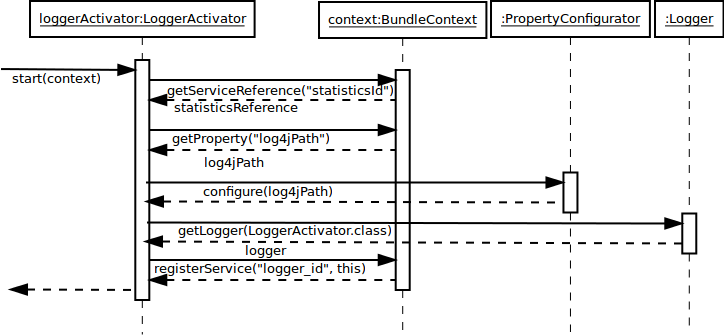
\includegraphics[scale=0.5]{img/sequence_logger}
\caption{A Logger komponens indulása}
\label{fig:sequence_logger}
\end{figure}

OSGi környezetben nem ilyen egyszerű az Apache log4j használata. Alapértelmezett esetben a log4j konfigurációs fájlját (log4j.properties) az alkalmazás gyökérkönyvtárába kell helyezni, OSGi környezetben nyilvánvaló módon ez nem működik. A legegyszerűbb megoldás fragment bundle készítése lenne, melynek nincs BundleActivator osztálya és megosztja classloaderét egy szülő komponenssel. Ennek azonban nagy hátránya van és az Apache log4j egyik előnyét veszítenénk el, mert fragment bundle készítésénél a konfigurációs fájlt a forráskóddal együtt be kellene csomagolni a komponensbe. Így nem lesz konfigurálható a naplózás formája, szintjei, be lesz égetve egy bundle-be minden beállítás.

A fenti hátrányokat elkerülhetjük, ha runtime property-ként megadjuk a helyét a merevlemezen tárolt log4j.properties fájlnak a Felix konfigurációjában. A naplózás beállítását egy szöveges fájlban leírhatjuk és azt a rendszerben bárhol elhelyezhetjük. Az Apache log4j beállítását és OSGi szolgáltatásként való kiajánlását a komponens indulásakor kell megtennünk (\ref{fig:sequence_logger}.~ábra).

% section loggerbundle (end)

\section{Statistics bundle}
\label{sec:statisticsbundle}

A Statistics komponens implementálásakor tehát két servletet és egy adatokat gyüjtő és tárolót kellett létrehozni. A tároló felépítése nagyon egyszerű, a tervezéskor meghatározott metrikákat reprezentáló adatokat tárolja attribútumokban, és implementálja egy kiajánlott OSGi szolgáltatás által meghatározott metrikák módosítására és lekérdezésére szolgáló metódusokat.

A servletek készítése egy kicsit bonyolultabb volt, mert ahhoz, hogy a servlet HTTP-n keresztül elérhető legyen be kell regisztrálni egy servlet container-be. A JEE/J2EE fejlesztés során megszokott web.xml fájlon keresztüli konfigurációt nem használhatjuk, OSGi környezetben, ezért az org.osgi.util.tracker.ServiceTracker osztályban kell beregisztrálnunk servletünket. Ehhez az előbbi osztályból kellett leszármaztatni egy osztályt (HttpServiceTracker a \ref{fig:class_statistics}.~ábrán) és felülírni az addingService és removedService metódusait, ahol be kellett regisztrálni a servlet osztályokat.

\begin{lstlisting}[label={lst:apidata}, caption=A WikiprocessorAPI által szolgáltatott adatok,breaklines=true]
{"articlesData":{"eltárolt cikkek száma":2785,"frissített cikkek száma":877,"újonnan beillesztett cikkek száma":1908,"nem feldolgozott cikkek száma":13},
"logsData":{"error üzenetek száma":3,"warning üzenetek száma":11,"debug üzenetek száma":4},
"queuelength":6013,"mainworkingparsoids":0.5714285714285714,"dumpworkingparsoids":0.8,"dumpprocess":0.11469880217730487}
\end{lstlisting}

A WikiprocessorAPI servlet a metrikák alapján JSON formátumban teszi közzé a feldolgozólánc adatait, így ez a servlet gyakorlatilag egy webes API-nak tekinthető. A StatisticsView egy statikus HTML oldalt szolgál ki, ahol az előbbi API-t felhasználva JavaScript segítségével diagramokat rajzol ki a servlet. A létrehozott diagramok a metrikákat alakítják a felhasználók számára sokkal jobban megfigyelhető formába.

% section statisticsbundle (end)

% chapter implementation (end)